\section{遗传算法}
\label{sec:rs-ga}

演化策略的搜索分布依赖连续变量的高斯结构，换到开关选择或排列上就用不上了。于是要问：候选是离散的编码时，怎样利用一批已评价的候选产生新的候选？\term{遗传算法}（genetic algorithm，GA）的做法是：维护一个种群，用评价选出亲代，把亲代的编码拼接和改动，得到新的候选。

“基因”“繁殖”只是沿用下来的名称。这些类比并不告诉我们一个操作在实际问题上做了什么。下面把四件事分开说明：候选的编码、亲代的选择、新候选的产生、下一代的组成。

\subsection{候选解的编码}
\label{sec:rs-ga-encoding}

遗传算法的操作都作用在编码上。这一小节的问题是：候选应当怎样写成编码，编码与原问题的解是什么关系？

\paragraph{选择问题：0--1串}
全节用一个背包问题作例子。有六件物品，第$j$件价值$v_j$、重量$w_j$，容量为$15$：
\[
 \bm{v}=(6,5,8,9,6,7),\qquad\bm{w}=(2,3,6,7,5,9).
\]

用串$\bm{b}\in\{0,1\}^6$表示选择，$b_j=1$表示选第$j$件。要最小化的是价值的相反数：
\begin{equation}
 f(\bm{b})=-\sum_{j=1}^{6}v_jb_j,\qquad\text{约束}\quad\sum_{j=1}^{6}w_jb_j\leq15.
 \label{eq:rs-knapsack}
\end{equation}
例如$\bm{b}=101100$选第$1,3,4$件，总重$15$，$f=-23$。穷举全部$2^6=64$个串可知这正是最优解，总共$30$个可行串。

\term{解码}（decoding）是从编码回到原问题的解，评价永远在解码之后进行。这里编码与解是一一对应的，解码平凡，但重量约束使得并非每个串都可行，第~\ref{sec:rs-constraints}节处理这一点。

\paragraph{顺序问题：排列}
访问顺序、任务排程的自然编码是排列，第~\ref{sec:rs-space}节的$ABDCE$就是一个例子，排列本身就是解。

把排列硬写成二进制会带来麻烦。五个元素每个用三位表示，一共$15$位，有$2^{15}=32768$种串，其中只有$5!=120$种是合法排列，约占$0.37\%$。翻一位多半得到重复元素的串，算法大部分精力花在非法候选上。

\paragraph{连续变量}
连续变量可以直接用实数向量编码，第~\ref{sec:rs-evaluation}节的比较实验就是这样做的，这时“交叉”是两个实数向量的组合，“变异”是加一个小扰动。

编码决定了什么叫“邻近”，决定了哪些操作合法，所以不存在一种通用的串表示。写清楚编码的含义、解码方式和合法操作，是这类算法要做的第一件事。

\subsection{亲代选择}
\label{sec:rs-ga-parents}

有了种群和评价，下一个问题是：谁来产生下一代的候选？选得太偏向好个体，种群很快只剩少数几种；选得太平均，又等于随机游走。用同一组数比较几种规则。设种群有$N=5$个候选，代价从好到差为
\begin{equation}
 (f_{1:5},\ldots,f_{5:5})=(-24,-20,-19,-15,-10).
 \label{eq:rs-selection-costs}
\end{equation}

\paragraph{排序选择}
把候选按代价排序，只按名次分配概率。线性排序取参数$s\in(1,2]$，第$r$名被选中的概率是
\begin{equation}
 p_r=\frac{1}{N}\Bigl(2-s+2(s-1)\frac{N-r}{N-1}\Bigr).
 \label{eq:rs-rank-selection}
\end{equation}
$s=1.5$，$N=5$时，五个名次的概率是
\[
 (0.30,\ 0.25,\ 0.20,\ 0.15,\ 0.10).
\]
由于只用名次，把代价做单调变换不影响选择。

\paragraph{锦标赛选择}
\term{锦标赛选择}（tournament selection）每次有放回地抽$k$个候选，选其中代价最小的。它不需要排序全体，也只用比较结果。第$r$名被选中，当且仅当这$k$次抽样都不比第$r$名更好（共有$N-r+1$个这样的候选可抽），并且至少有一次抽到了第$r$名。所以
\begin{equation}
 p_r=\frac{(N-r+1)^k-(N-r)^k}{N^k}.
 \label{eq:rs-tournament}
\end{equation}
这里默认没有并列。

$N=5$，$k=2$时，五个名次的概率是
\[
 (0.36,\ 0.28,\ 0.20,\ 0.12,\ 0.04).
\]

$k=3$时是
\[
 (0.488,\ 0.296,\ 0.152,\ 0.056,\ 0.008).
\]
$k$越大，好候选被选中的倾向越强。这种倾向称为\term{选择压力}（selection pressure）。以第$1$名在$N$次选择中的期望份数$Np_1$度量，$k=2$时是$1.8$份，$k=3$时是$2.44$份。

\paragraph{比例选择要先转换}
经典的比例选择把选中概率设为正比于\term{适应度}（fitness）$F$。最小化问题的代价不能直接拿来用：代价越低越好，比例却是数越大份额越大，方向就是反的。

把式~\eqref{eq:rs-selection-costs}的代价都加上$20$，问题没有变，五个数成为$(-4,0,1,5,10)$，总和是$12$，第一个比值是负数，根本不是概率。

必须先指定从代价到非负权重的转换。一种做法是以当前最差者为基准：
\begin{equation}
 F_i=f_{\max}-f_i+\delta,\qquad\delta>0.
 \label{eq:rs-fitness}
\end{equation}
取$\delta=1$，得到权重$(15,11,10,6,1)$，总和为$43$，五个概率约为
\[
 (0.349,\ 0.256,\ 0.233,\ 0.140,\ 0.023).
\]

这个转换对代价的平移不变，但概率依赖代价差的相对大小，也依赖$\delta$的取值，把$\delta$取大，选择会趋于均匀。图~\ref{fig:rs-ga-selection}把几种规则画在一起。

\begin{BookInlineFigure}
 \centering
 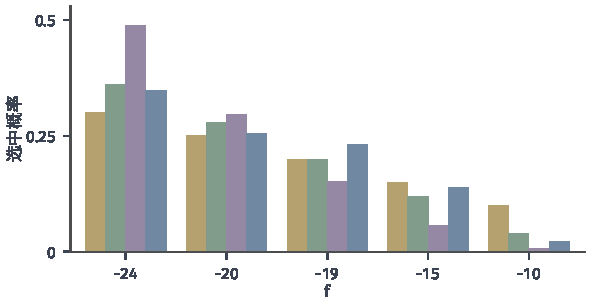
\includegraphics[width=100mm]{figures/05-optimization/05-stochastic-optimization/matplotlib/rs-ga-selection/figure.pdf}
 \caption{同一组代价~\eqref{eq:rs-selection-costs}下五个候选的选中概率，从左到右依次为线性排序（黄，$s=1.5$）、二元锦标赛（绿）、三元锦标赛（紫）、比例选择（蓝，$\delta=1$）。}
 \label{fig:rs-ga-selection}
\end{BookInlineFigure}

\subsection{交叉与变异}
\label{sec:rs-ga-operators}

选出亲代以后，怎样产生新候选？有两种操作，职责不同。\term{交叉}（crossover）把两个亲代已有的片段重新组合，只能产生两个亲代片段的拼接。\term{变异}（mutation）改动个别位置，引入亲代都没有的内容。

\paragraph{二进制串}
\textbf{单点交叉}随机选一个切点，交换切点后的尾部。用两个亲代
\[
 \bm{a}=110\,100,\qquad\bm{b}=101\,010,
\]
切点在第$3$位之后。

$\bm{b}$的前三位接$\bm{a}$的后三位，得到$101\,100$；$\bm{a}$的前三位接$\bm{b}$的后三位，得到$110\,010$。第一个后代正是最优解$101100$，$f=-23$，比两个亲代的$-20$都好。第二个后代$110010$总重$10$，$f=-17$，比两个亲代都差。交叉只是重新组合，不保证任何一个后代更好。

\textbf{逐位变异}对每一位独立以概率$p_m$翻转，常取$p_m=1/n$，平均每个串翻一位。图~\ref{fig:rs-ga-crossover}(a)中第二个后代的第$4$位翻转，变成$110110$。这个串总重$17$，超过容量，是不可行的。

\begin{BookInlineFigure}
 \centering
 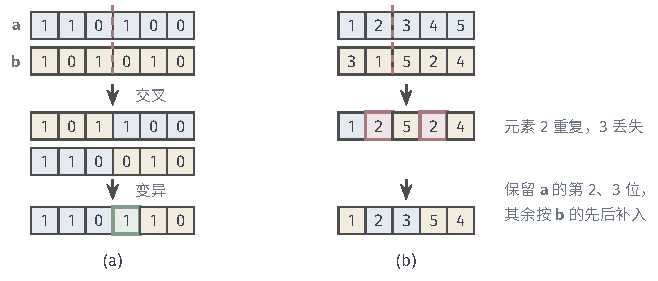
\includegraphics[width=111mm]{figures/05-optimization/05-stochastic-optimization/tikz/rs-ga-crossover/figure.pdf}
 \caption{二进制串与排列上的操作。蓝色格来自亲代$\bm{a}$，黄色格来自亲代$\bm{b}$，红色虚线是切点。(a)单点交叉后，第二个后代的第$4$位变异（绿框）。(b)在排列上直接交换尾部会产生重复元素（红框）；保留$\bm{a}$的中段再按$\bm{b}$的先后顺序补入其余元素，得到合法排列。}
 \label{fig:rs-ga-crossover}
\end{BookInlineFigure}

\paragraph{排列要用保持排列的算子}
排列上的单点交叉会出错。$\bm{a}=12345$，$\bm{b}=31524$，切点在第$2$位之后，直接拼接得到$12\,524$，元素$2$出现两次，元素$3$丢失，已经不是排列。

有两种处理办法：换用保持排列的算子，或者明确规定修复规则。\textbf{顺序交叉}属于前者：保留$\bm{a}$的第$2$、$3$位，即$23$，其余位置按$\bm{b}$中出现的先后依次填入尚未使用的元素，$\bm{b}$的顺序去掉$2,3$后是$1,5,4$，于是得到$12354$。排列上的变异也用交换两个位置或翻转一段，而不用单独改一个位置。

\paragraph{两组参数分开记录}
交叉概率$p_c$是一对亲代发生交叉的概率，不交叉时后代直接复制亲代。变异概率$p_m$是每一位翻转的概率，作用范围是一位而不是一个串。两者要分别记录。

两种操作各自都不保证改善目标。上面的例子里，同一次交叉同时给出了最好的和较差的后代，一次变异把后代变得不可行。质量的提升要靠后面的选择来累积。

\subsection{后代替换}
\label{sec:rs-ga-replacement}

亲代选择决定谁来产生新候选，后代替换决定谁进入下一代，两者是两个独立的决定。

\paragraph{三种替换}
\textbf{整代替换}用后代完全替代上一代。\term{精英保留}（elitism）在整代替换的基础上把上一代最好的若干个直接带入下一代。\textbf{逐个替换}每产生一个后代，就让它替换当前种群中最差的个体，如果它比那个个体好的话。

\needspace{6\baselineskip}
\paragraph{变量}
下面在背包问题上走完一代。要维护的量是：
\begin{itemize}
 \item 种群$\bm{b}_1,\ldots,\bm{b}_N$及其代价，$N$是种群规模；
 \item 历史最好可行解及其代价。
\end{itemize}

\paragraph{初始化}
产生初始种群并评价，这一步消耗$N$次评价。例中$N=4$，初始种群是
\[
 \begin{gathered}
 A=110100\ (\text{重}12,\ f=-20),\qquad B=101010\ (\text{重}13,\ f=-20),\\
 C=011010\ (\text{重}14,\ f=-19),\qquad D=100110\ (\text{重}14,\ f=-21).
 \end{gathered}
\]
最好记录是$D$，代价$-21$。超重的串在选择时用罚项代价$f+10\times$（超重量），第~\ref{sec:rs-constraints}节再比较其他做法。

\paragraph{每轮更新}
每一代重复以下步骤，直到预算用完。

\begin{enumerate}
 \item 用二元锦标赛选两个亲代。例中第一次比较$(B,C)$，胜者$B$；第二次比较$(A,C)$，胜者$A$。
 \item 按$p_c$决定是否交叉。例中切点在第$3$位之后，得到$101100$和$110010$。
 \item 按$p_m$逐位变异。例中第一个后代不变，第二个后代第$4$位翻转，成为$110110$。
 \item 解码并评价后代，更新历史最好可行解。例中$101100$总重$15$，$f=-23$，可行，记录更新。$110110$总重$17$，价值$26$，$f=-26$，超重$2$，罚项代价为
 \[
  -26+10\times2=-6.
 \]
 这个串的$f$虽低，却不能进入可行解的记录。
 \item 重复第1到4步，直到得到$N$个后代。例中第二对亲代的比较为$(D,A)$，胜者$D$；$(C,C)$抽到同一个候选，$C$胜出。切点在第$2$位之后，无变异，得到$101010$（$f=-20$）和$010110$（重$15$，$f=-20$）。
 \item 组成下一代。整代替换时下一代是这四个后代；精英保留一个时，$D$取代后代中最差的$110110$。
\end{enumerate}

这一代消耗$4$次评价。最终得到历史最好可行解$101100$，它是这个问题的最优解。

三种替换的结果放在表~\ref{tab:rs-ga-replacement}中。这次后代中有更好的解，三种规则的最好值都是$-23$；差别在于下一代的其余成员。如果这一代的后代都很差，整代替换会使种群的最好值变差，精英保留和逐个替换不会。

\begin{BookInlineTable}
 \centering
 \caption{同一代的三种替换结果，第三列是对应的选择用代价。}
 \label{tab:rs-ga-replacement}
 \begin{tabular}{lll}
  \toprule
  规则 & 下一代 & 代价 \\
  \midrule
  整代替换 & $101100,110110,101010,010110$ & $-23,-6,-20,-20$ \\
  精英保留 & $101100,100110,101010,010110$ & $-23,-21,-20,-20$ \\
  逐个替换 & $110100,101010,101100,100110$ & $-20,-20,-23,-21$ \\
  \bottomrule
 \end{tabular}
\end{BookInlineTable}

逐个替换那一行的过程是：$101100$替换当时最差的$C(-19)$；$110110$的$-6$比当前最差的$-20$差，不替换；后两个后代的$-20$与最差者持平，规定严格更好才替换，所以也不替换。

\paragraph{多样性的丢失}
种群有一个专门的失败方式：所有成员越来越像。把多样性度量为种群中两个不同成员平均相差的位数占总位数的比例。若某一位全种群都相同，交叉再怎么拼接，这一位也不会改变，只有变异才能恢复。

图~\ref{fig:rs-ga-diversity}在一个$40$件物品的背包问题上比较两种变异率，种群$N=30$，二元锦标赛，单点交叉，精英保留一个。没有变异时，多样性约$20$代内降到$0$，种群变成同一个串，此后每一代的后代都与亲代相同，相对最优值的间隙卡在约$15\%$。变异率$1/40$时多样性稳定在约$0.2$，$150$代后间隙约为$1.4\%$。

\begin{BookInlineFigure}
 \centering
 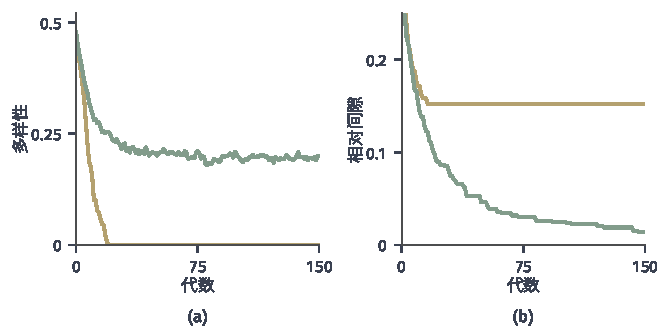
\includegraphics[width=112mm]{figures/05-optimization/05-stochastic-optimization/matplotlib/rs-ga-diversity/figure.pdf}
 \caption{$40$件物品的背包问题，$31$次运行的中位数。黄线不变异，绿线变异率$1/40$。(a)种群多样性，即两个不同成员平均相差的位数占总位数的比例。(b)历史最好可行解与最优价值的相对间隙，最优价值由动态规划算出。}
 \label{fig:rs-ga-diversity}
\end{BookInlineFigure}

保持多样性的手段有三个：变异持续注入新内容；较大的种群让位点的多样性丢失得慢；种群收敛后保留最好记录并重启。它们都消耗评价次数，要在预算内权衡。

精英保留也不能提供有限预算下的全局保证。它只保证种群的最好值不变差，这和第~\ref{sec:rs-es-selection}节的结论相同，精英甚至可能加速多样性的丢失，因为它的片段被反复选中。
